\documentclass[tikz,svgnames]{standalone}

\usetikzlibrary{backgrounds}

\begin{document}

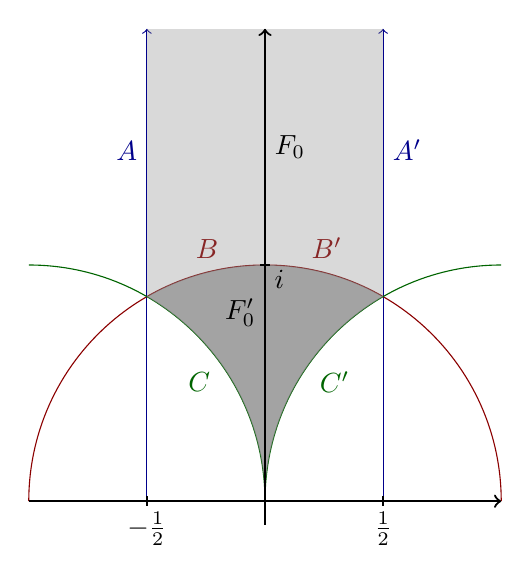
\begin{tikzpicture}[scale=3]
  \def\xmin{-1} \def\xmax{1}
  \def\ymin{-0.1} \def\ymax{2}

  \draw [thick,->] (\xmin,0) -- (\xmax,0);
  \draw [thick,->] (0,\ymin) -- (0,\ymax);

  \draw [thick] (-0.5,-0.02) -- (-0.5,0.02) node [below=2] {$-\frac{1}{2}$};
  \draw [thick] (0.5,-0.02) -- (0.5,0.02) node [below=2] {$\frac{1}{2}$};
  \draw [thick] (-0.02,1) -- (0.02,1) node [below right=-2] {$i$};
  \node at (0,3*\ymax/4) [right] {$F_0$};
  \node at (0,0.8) [left] {$F_0^\prime$};

  \begin{pgfonlayer}{background}
    \draw [DarkBlue,->] (-0.5,0) -- (-0.5,\ymax) node [pos=0.7,above left] {$A$};
    \draw [DarkBlue,->] (0.5,0) -- (0.5,\ymax) node [pos=0.7,above right] {$A^\prime$};
    \draw [DarkRed] (1,0) arc (0:180:1) node [auto,swap,pos=0.55] {$B$} node [auto,swap,pos=0.45] {$B^\prime$};
    \draw [DarkGreen] (0,0) arc (0:90:1) node [auto,pos=0.4] {$C$};
    \draw [DarkGreen] (1,1) arc (90:180:1) node [auto,pos=0.6] {$C^\prime$};

    \path[clip] (1,\ymax) -- (1,1) arc (90:180:1) -- (0,0) arc (0:90:1) -- (-1,\ymax) -- cycle;

    \begin{scope}
      \path[clip] (1,\ymax) -- (1,1) arc (90:180:1) -- (0,0) arc (0:90:1) -- (-1,\ymax) -- cycle;
      \fill[gray,opacity=0.3] (-0.5,0) rectangle (0.5,\ymax);
      \fill[gray,opacity=0.6] (1,0) arc (0:180:1);
    \end{scope}
  \end{pgfonlayer}
\end{tikzpicture}

\end{document}
